%=======================================================================================%
\chapter{Molecular Dynamics and Theratyping in Airway and Gut Organoids Reveal R352Q-CFTR Conductance Defect}
\label{chap:R352Q}
\chapquote{Cells have a mind of their own} {-Shafagh Waters (personal communication)}

\section*{\centering Abstract} 
A significant challenge to making targeted CFTR modulator therapies accessible to all individuals with cystic fibrosis (CF) are many mutations in the CFTR gene that can cause CF, most of which remain uncharacterized. Here, we characterized the structural and functional defects of the rare CFTR mutation R352Q – with potential role contributing to intrapore chloride ion permeation – in patient-derived cell models of the airway and gut. CFTR function in differentiated nasal epithelial cultures and matched intestinal organoids was assessed using ion transport assay and forskolin-induced swelling (FIS) assay respectively. CFTR potentiators (VX-770, GLPG1837 and VX-445) and correctors (VX-809, VX-445 +/- VX-661) were tested.  Data from R352Q-CFTR were compared to that of twenty participants with mutations with known impact on CFTR function. R352Q-CFTR has residual CFTR function which was restored to functional CFTR activity by CFTR potentiators but not the corrector. Molecular dynamics (MD) simulations of R352Q-CFTR were carried out which indicated the presence of a chloride conductance defect, with little evidence supporting a gating defect. The combination approach of in vitro patient-derived cell models and in silico MD simulations to characterize rare CFTR mutations can improve the specificity and sensitivity of modulator response predictions and aid in their translational use for CF precision medicine.


\smallskip
%\begin{figure*} [h]
%	\begin{center}
%		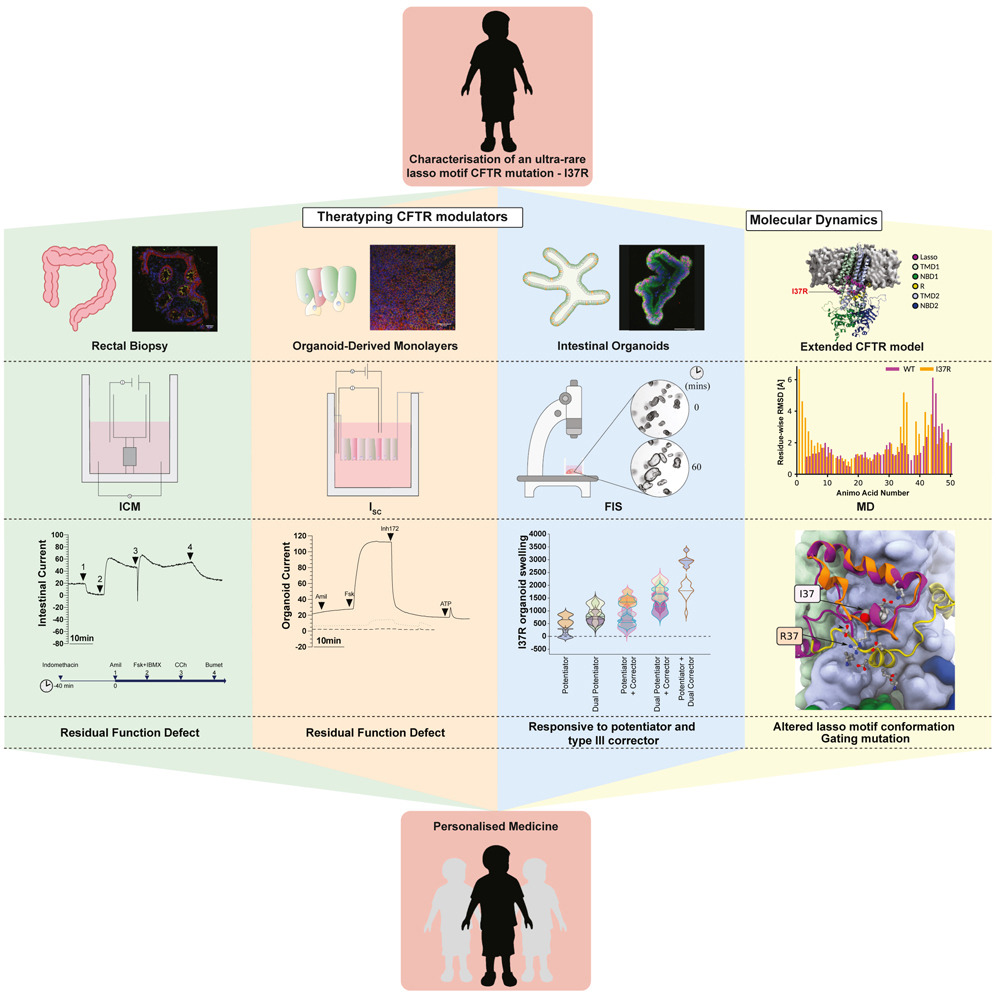
\includegraphics[width=0.80\textwidth]{figures/I37R/graphical_abstract.jpg}
%	\end{center}
%	\captionsetup{singlelinecheck = false, justification=raggedright}
%	\caption[Graphical Abstract. Integration of in silico and in vitro experiments for personalised medicine] {\textbf{Graphical Abstract. Integration of in silico and in vitro experiments for personalised medicine}}{}
%	\label{I37R_graphical_abstract}
%\end{figure*}

\section{Introduction}
Cystic fibrosis (CF), a rare, life-limiting disorder affecting $\sim$90,000 individuals worldwide \cite{rasaruseckaite2017}, results from a malfunction in the cystic fibrosis transmembrane conductance regulator (CFTR) protein. CFTR functions as a cAMP-stimulated anion channel \cite{saint-criq2017}. Chloride ions diffuse through the CFTR channel pore, causing a charge imbalance that is corrected by the flux of sodium ions through sodium channels \cite{saint-criq2017}. The resultant ion imbalance causes osmosis of water into the extracellular space. More than 2,000 variants in the CFTR gene are known. CFTR mutations are grouped into six major classes based on their functional defects in protein synthesis (I); intracellular maturation, processing, or folding (II); channel gating (III) or conductance activity (IV); diminished quantity (V); and diminished stability (VI) \cite{marson2016}.

CFTR modulators can restore mutant CFTR protein function \cite{clancy2019}. Two subclasses of modulators are in current clinical use, though approval varies between countries. Potentiators such as ivacaftor (VX-770|Kalydeco; Vertex Pharmaceuticals) increase CFTR channel gate opening. Correctors such as lumacaftor (VX-809), tezacaftor (VX-661), and elexacaftor (VX-445) increase delivery of misfolded CFTR to the cell surface. VX-809 and VX-661 are type I correctors that work by stabilizing the NBD1–TMD1 and/or NBD1–TMD2 interface by binding directly to TMD1 \cite{loo2013, ren2013}. VX-445 is a type III corrector that directly stabilizes NBD1 and has been shown to have copotentiator activity \cite{shaughnessy2021, laselva2021, veit2021a, okiyoneda2013}. Combination therapies of potentiator and corrector(s) (Orkambi, Symdeko, Trikafta; Vertex Pharmaceuticals) are approved for use in patients with CF homozygous for F508del, the most common CFTR mutation\cite{commissioner2020, fda_symdeko_approval, fda_orkambi_approval}. Trikafta is also approved for patients with CF who are heterozygous for F508del \cite{commissioner2020}. The remaining patients with CF are either compound heterozygous or homozygous for mutations other than F508del, only some of which are approved for treatment with modulator therapy \cite{fda_expansion_rare_mutations}. A large number of CFTR mutations are not approved for modulator therapy, because their exact mechanism of CFTR dysfunction and/or responsiveness to modulator therapy is often unknown. Traditional randomized clinical trials of modulators to identify modulator-responsive patients with CF with rare CFTR mutations are costly, time-consuming, and impractical \cite{bell2020}.

A major breakthrough in the field of CF has been the development of two preclinical patient- and organ-specific cell models \cite{clarke2013, dekkers2016a, martinovich2017}. Both models are used in functional assays that allow rapid quantitative measurements of CFTR function. Differentiated airway epithelial cells are used in transepithelial ion transport assays (short circuit current [Isc]) \cite{pranke2017}. Intestinal organoids are used in forskolin (Fsk)-induced swelling (FIS) assays \cite{dekkers2013a}. Each serves as a personalized functional model of the patient’s CFTR mutation and response to modulators. However, how cell models of the airway compare with those of the gut created from the same patient is not well understood. Mean changes in CFTR function in vivo correlate with the CFTR rescue assessed via the Isc and FIS assays in cell models of subjects with the same mutations \cite{dekkers2016a, pranke2017}. In addition, cell model responses in subjects with ultrarare mutations have successfully predicted clinical benefit \cite{ramalho2021, mccarthy2018, berkers2019}. Results so far support the use of patient-derived cell models to guide personalized treatment \cite{pranke2019a}.

We established human nasal epithelial cell (hNEC) cultures from 11 participants with wild-type functioning CFTR (WT/WT) and 10 participants with CF. The participants with CF included five participants with known and characterized CFTR folding/maturation defects (F508del/F508del), three with a CFTR synthesis defect (G542X/F508del), and one with a CFTR gating defect (G551D/F508del). The results from these CFTR mutations with a known impact on CFTR function were used as a reference and were compared with the results from one participant with the R352Q/F508del CFTR genotype. We also created matched intestinal organoids from seven participants with CF and one WT-CFTR control participant (see Table E1 in the data supplement). R352Q, a rare CFTR mutation in the CFTR channel pore, was chosen because it has been characterized in heterologous systems but is yet to be tested in a patient-derived model. Single-channel and whole-cell patch-clamp studies have demonstrated R352 to be a molecular determinant of anion selectivity and permeability in the CFTR channel pore \cite{guinamard1999}. Our aims were to assess CFTR baseline activity and CFTR modulator response in Isc and FIS assays. Potentiator agents VX-770 and GLPG1837 (a potentiator in clinical trials; hereafter G1837) were tested individually and in combination with a CFTR protein-folding corrector VX-809. The effect of VX-445 as a potentiator (acute treatment) and corrector (chronic treatment) monotherapy, as well as part of triple combination therapy VX-445+VX-661+VX-770 (Trikafta) were assessed in FIS assays. In addition, to gain a complementary and better understanding of the effect of R352Q mutation on CFTR function, in silico structural atomistic modeling and molecular dynamics simulations were performed. Some of the results of these studies have been reported previously in the form of a preprint (\href{https://doi.org/10.1101/2021.08.11.456003}{https://doi.org/10.1101/2021.08.11.456003}).


\section{Results}
\subsection{R352Q-CFTR Baseline Activity and Response to CFTR Modulators in Nasal Epithelial Cells}
Mature, differentiated hNECs were pseudostratified (Figure 1A) and had functional beating cilia (CBF, 6.2 $\pm$ 0.1 Hz) (Figure 1B, Video 1) and intact junction integrity (Figure 1A) (transepithelial electrical resistance, $\geq$170 $\Omega\cdot$cm$^2$; Figure E1A). To assess ion transport, Isc measurements were performed (Figures E1B–E1D). We first determined the CFTR activity threshold in reference cell models, which were used for comparison with R352Q-CFTR functional activity before and after modulator stimulation. Fsk-stimulated CFTR-dependent anion currents ($\Delta$Isc-Fsk) in WT/WT hNECs were 21.2 $\pm$ 1.2 $\mu$A/cm$^2$ at baseline (Figures 1C and 1D, Table E2). Baseline $\Delta$Isc-Fsk in F508del/F508del hNECs was at 3.4 $\pm$ 0.5 $\mu$A/cm$^2$ and was not increased beyond ~0.8 $\mu$A/cm$^2$ with either potentiator (Figure 1D). Because of the presence of two copies of the same CFTR mutation, we considered that protein expression from each of the F508del alleles was likely to be the same and therefore attributed each allele to equally contribute ~1.7 $\mu$A/cm$^2$ to baseline Fsk-stimulated currents and ~0.4 $\mu$A/cm$^2$ to potentiator-stimulated currents (Table E2). The baseline $\Delta$Isc-Fsk of G542X/F508del hNECs was 0.81 $\pm$ 0.12 $\mu$A/cm$^2$. Because G542X is a synthesis defect mutation with no functional CFTR protein production, the observed ~0.81 $\mu$A/cm$^2$ is attributed to the F508del allele, which is not considerably different from that calculated from the F508del/F508del hNECs. We thus used these values as a guide to estimate the contribution of the F508del allele to the experimental Isc data of the heterozygous R352Q/F508del participant. In support of this, F508del/WT hNECs were previously shown to have, on average, ~50\% of Fsk-stimulated currents of WT/WT hNECs, although variability between F508del/WT participants was present \cite{pranke2017}.


%\begin{figure*} 
	\begin{center}
		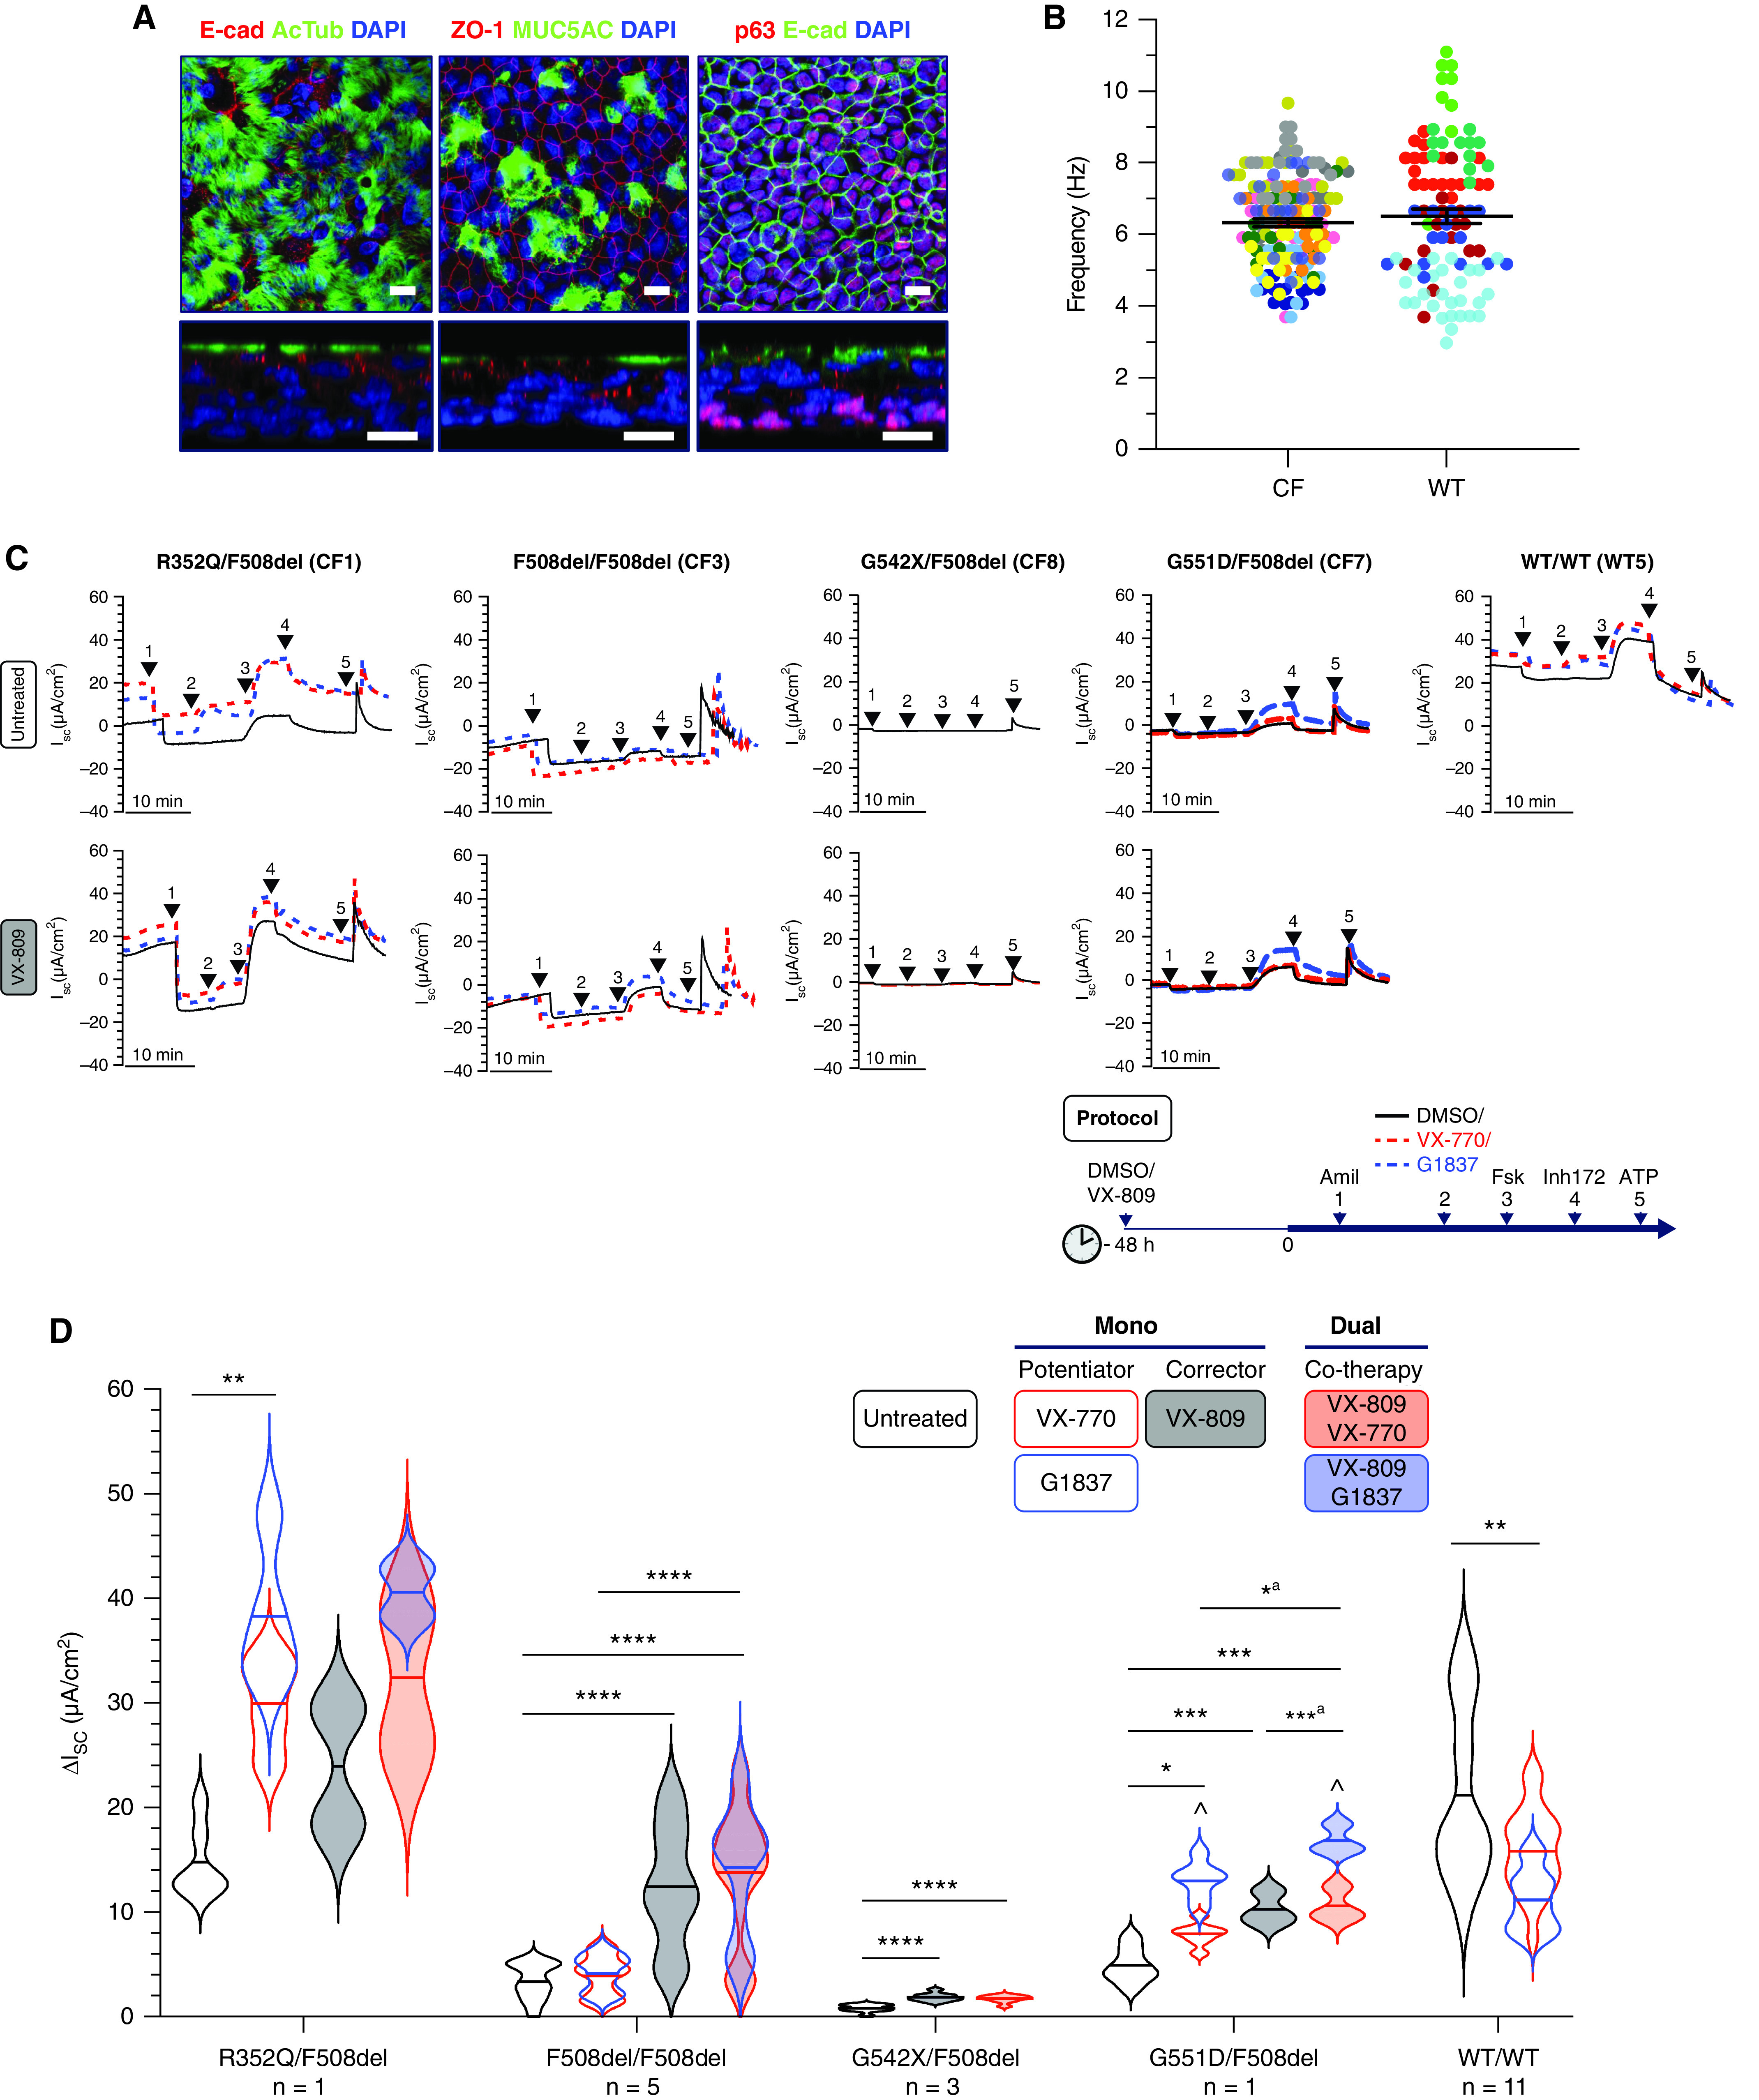
\includegraphics[width=0.80\textwidth]{figures/R352Q/figure_1.jpg}
	\label{R352_figure_1}
	\end{center}
	%\captionsetup{singlelinecheck = false, justification=raggedright}
	\begingroup
	\captionof{figure}[Functional response of R352Q-CFTR to cystic fibrosis transmembrane conductance regulator (CFTR) modulators in differentiated human nasal epithelial cells (hNECs). ] {\textbf{Functional response of R352Q-CFTR to cystic fibrosis transmembrane conductance regulator (CFTR) modulators in differentiated human nasal epithelial cells (hNECs). }}{(A) Immunofluorescence staining of acetylated tubulin (ciliated cells), MUC5AC (goblet cells), and p63 (basal progenitor cells) in hNECs derived from a R352Q/F508del participant (CF1). E-cadherin (adherens junction) and ZO-1 (tight junction) are localized to the intercellular junctions of epithelial cells. The top panels are top views and the bottom panels are side views showing the pseudostratified epithelium. A 63$\times$/1.4 numerical aperture oil immersion objective was used. Scale bars, 10 $\mu$m. (B) Dot plots of mean ciliary beat frequency (CBF) measurements (Hz) of the fully differentiated mature hNECs from participants with cystic fibrosis (CF) and without CF (wild type [WT]). Each participant is coded with a different color. Each dot represents a single field of view of CBF measurement. (C) Representative Ussing chamber recordings of short circuit current (Isc) in hNECs from participants with CF and WT-CFTR control participants. The protocol used to measure functional CFTR expression in hNECs in 0.01\% DMSO vehicle (untreated; top) or pretreated with corrector (3 $\mu$M VX-809 for 48 h; bottom) followed by sequential addition of 100 $\mu$M apical amiloride (1. Amil), apical addition of either vehicle control 0.01\% DMSO (black) or 10 $\mu$M VX-770 (red) or 10 $\mu$M G1837 (blue) (2. DMSO, VX-770, G1837), 10 $\mu$M basal forskolin (3. Fsk), 30 $\mu$M apical CFTR inhibitor (4. CFTRinh-172), and 100 $\mu$M apical ATP (5. ATP). A basolateral-to-apical chloride gradient was used. (D) Violin plots of total currents stimulated by DMSO or VX-770 or G1837 plus Fsk in hNECs untreated or pretreated with VX-809. Data are from 1 R352Q/F508del participant, 5 F508del/F508del participants, 3 G542X/F508del participants, and 1 G551D/F508del participant with CF and 11 WT-CFTR control participants. n, number of participants. Data are represented as violin plots to show the distribution of data. One-way ANOVA was used to determine statistically significant differences. *P $<$ 0.05, **P $<$ 0.01, ***P $<$ 0.001, and ****P $<$ 0.0001. aP for G1837 only. \^P for G1837 vs VX-770. Where VX-770 and G1837 (overlapping violin plots) both achieved statistical significance, the least significant P value is shown.}
	\endgroup
%\end{figure*}

R352Q/F508del hNECs demonstrated baseline CFTR activity of 14.8 $\pm$ 1.4 $\mu$A/cm$^2$, an appreciable 70\% of WT-CFTR activity (Figures 1C and 1D, Table E2). Potentiation with VX-770 or G1837 led to a significant (P $<$ 0.01) twofold increase in CFTR activity, reaching 15.2 and 23.5 $\mu$A/cm$^2$ above baseline, respectively (~140–180\% WT-CFTR activity). This response is similar to the potentiator-stimulated response observed in the reference gating G551D/F508del hNECs. The G551D/F508del hNECs had $\Delta$Isc-Fsk of 4.9 $\pm$ 0.6 $\mu$A/cm$^2$ at baseline, and treatment with either potentiator caused an approximately twofold increase in CFTR activity above baseline (net increase, VX-770, 3.0 $\mu$A/cm$^2$; G1837, 8.1 $\mu$A/cm$^2$) (Figures 1C and 1D, Table E2). The majority of the response to potentiators in R352Q/F508del hNECs was most likely contributed by the restored R352Q, because the total response is far greater than the 0.4 $\mu$A/cm$^2$ that we estimated to be attributed to the F508del allele (Figure 1D). We conclude that R352Q-CFTR has high baseline activity amenable to potentiator rescue in hNECs.

We next explored whether corrector monotherapy or cotherapy with potentiators increased R352Q-CFTR functional rescue. In F508del/F508del-CFTR cultures pretreated with VX-809, Fsk alone significantly (P $<$ 0.0001) enhanced CFTR-mediated Cl− currents by 3.7-fold, reaching 9.0 $\mu$A/cm$^2$ above baseline (Figures 1C and 1D, Table E2). We estimated each of the F508del alleles to equally contribute 4.5 $\mu$A/cm$^2$ to this increase in current. VX-809 cotherapy with either VX-770 or G1837 significantly (P $<$ 0.0001) increased the currents stimulated by potentiator monotherapy by ~10 $\mu$A/cm$^2$ (Figure 1D). In G542X/F508del hNECs, treatment with VX-809 resulted in a modest but significant (P $<$ 0.0001) increase in Fsk-stimulated currents by 1.04 $\mu$A/cm$^2$ above baseline (Figures 1C and 1D, Table E2). In G551D/F508del hNECs, VX-809 treatment significantly (P $<$ 0.001) increased CFTR activity by 5.4 $\mu$A/cm$^2$ above baseline (Figures 1C and 1D, Table E2). Because G551D mutation does not respond to VX-809 treatment \cite{han2018}, the contribution of the F508del allele was considered to be 5.4 $\mu$A/cm$^2$, similar to that calculated from the F508del/F508del hNECs. In addition, VX-809 cotherapy with either VX-770 or G1837 also increased the respective potentiator monotherapy currents by 2.7 $\mu$A/cm$^2$ and 3.8 $\mu$A/cm$^2$, respectively (Figure 1D). Unlike F508del/F508del-CFTR, the 9.1 $\mu$A/cm$^2$ increase in R352Q/F508del CFTR activity from the baseline in response to VX-809 monotherapy was not statistically significant (P = 0.09). VX-809 cotherapy with either potentiator also resulted in a nonsignificant increase in VX-770– or G1837-potentiated CFTR currents by ~2 $\mu$A/cm$^2$ (Figure 1D). Because VX-809 does not rescue R352Q, then R352Q-CFTR is unlikely to have a folding/maturation defect. The modest increase in current with VX-809 treatment was mostly if not fully imparted by the rescued F508del allele in the R352Q/F508del hNECs.

\subsection{R352Q-CFTR Baseline Activity and Response to CFTR Modulators in Intestinal Organoids}

We evaluated CFTR activity in matched intestinal organoids from the same participant with the R352Q/F508del genotype and those participants with reference F508del/F508del, G551D/F508del, and WT/WT genotypes using an FIS assay. To detect baseline and modulator-stimulated CFTR activity in the organoids, swelling was assessed at four Fsk concentrations ranging from 0.02 to 5 $\mu$M. FIS of organoids was dependent on Fsk dose, CFTR genotype, and the individual participant (Figure 2A). At 0.8 $\mu$M Fsk, the optimal concentration for baseline FIS assessment \cite{dekkers2016}, minimal swelling was observed for the F508del/F508del (area under the curve [AUC], 42.8 $\pm$ 19.4) and G551D/F508del organoids (AUC, 82.9 $\pm$ 20.1) (Figure 2A). R352Q/F508del and WT/WT organoids showed considerably higher FIS at the same 0.8 $\mu$M Fsk concentration, with AUCs of 196.3 $\pm$ 19.9 and 578.3 $\pm$ 61.6, respectively (Figure 2A).


	\begin{center}
		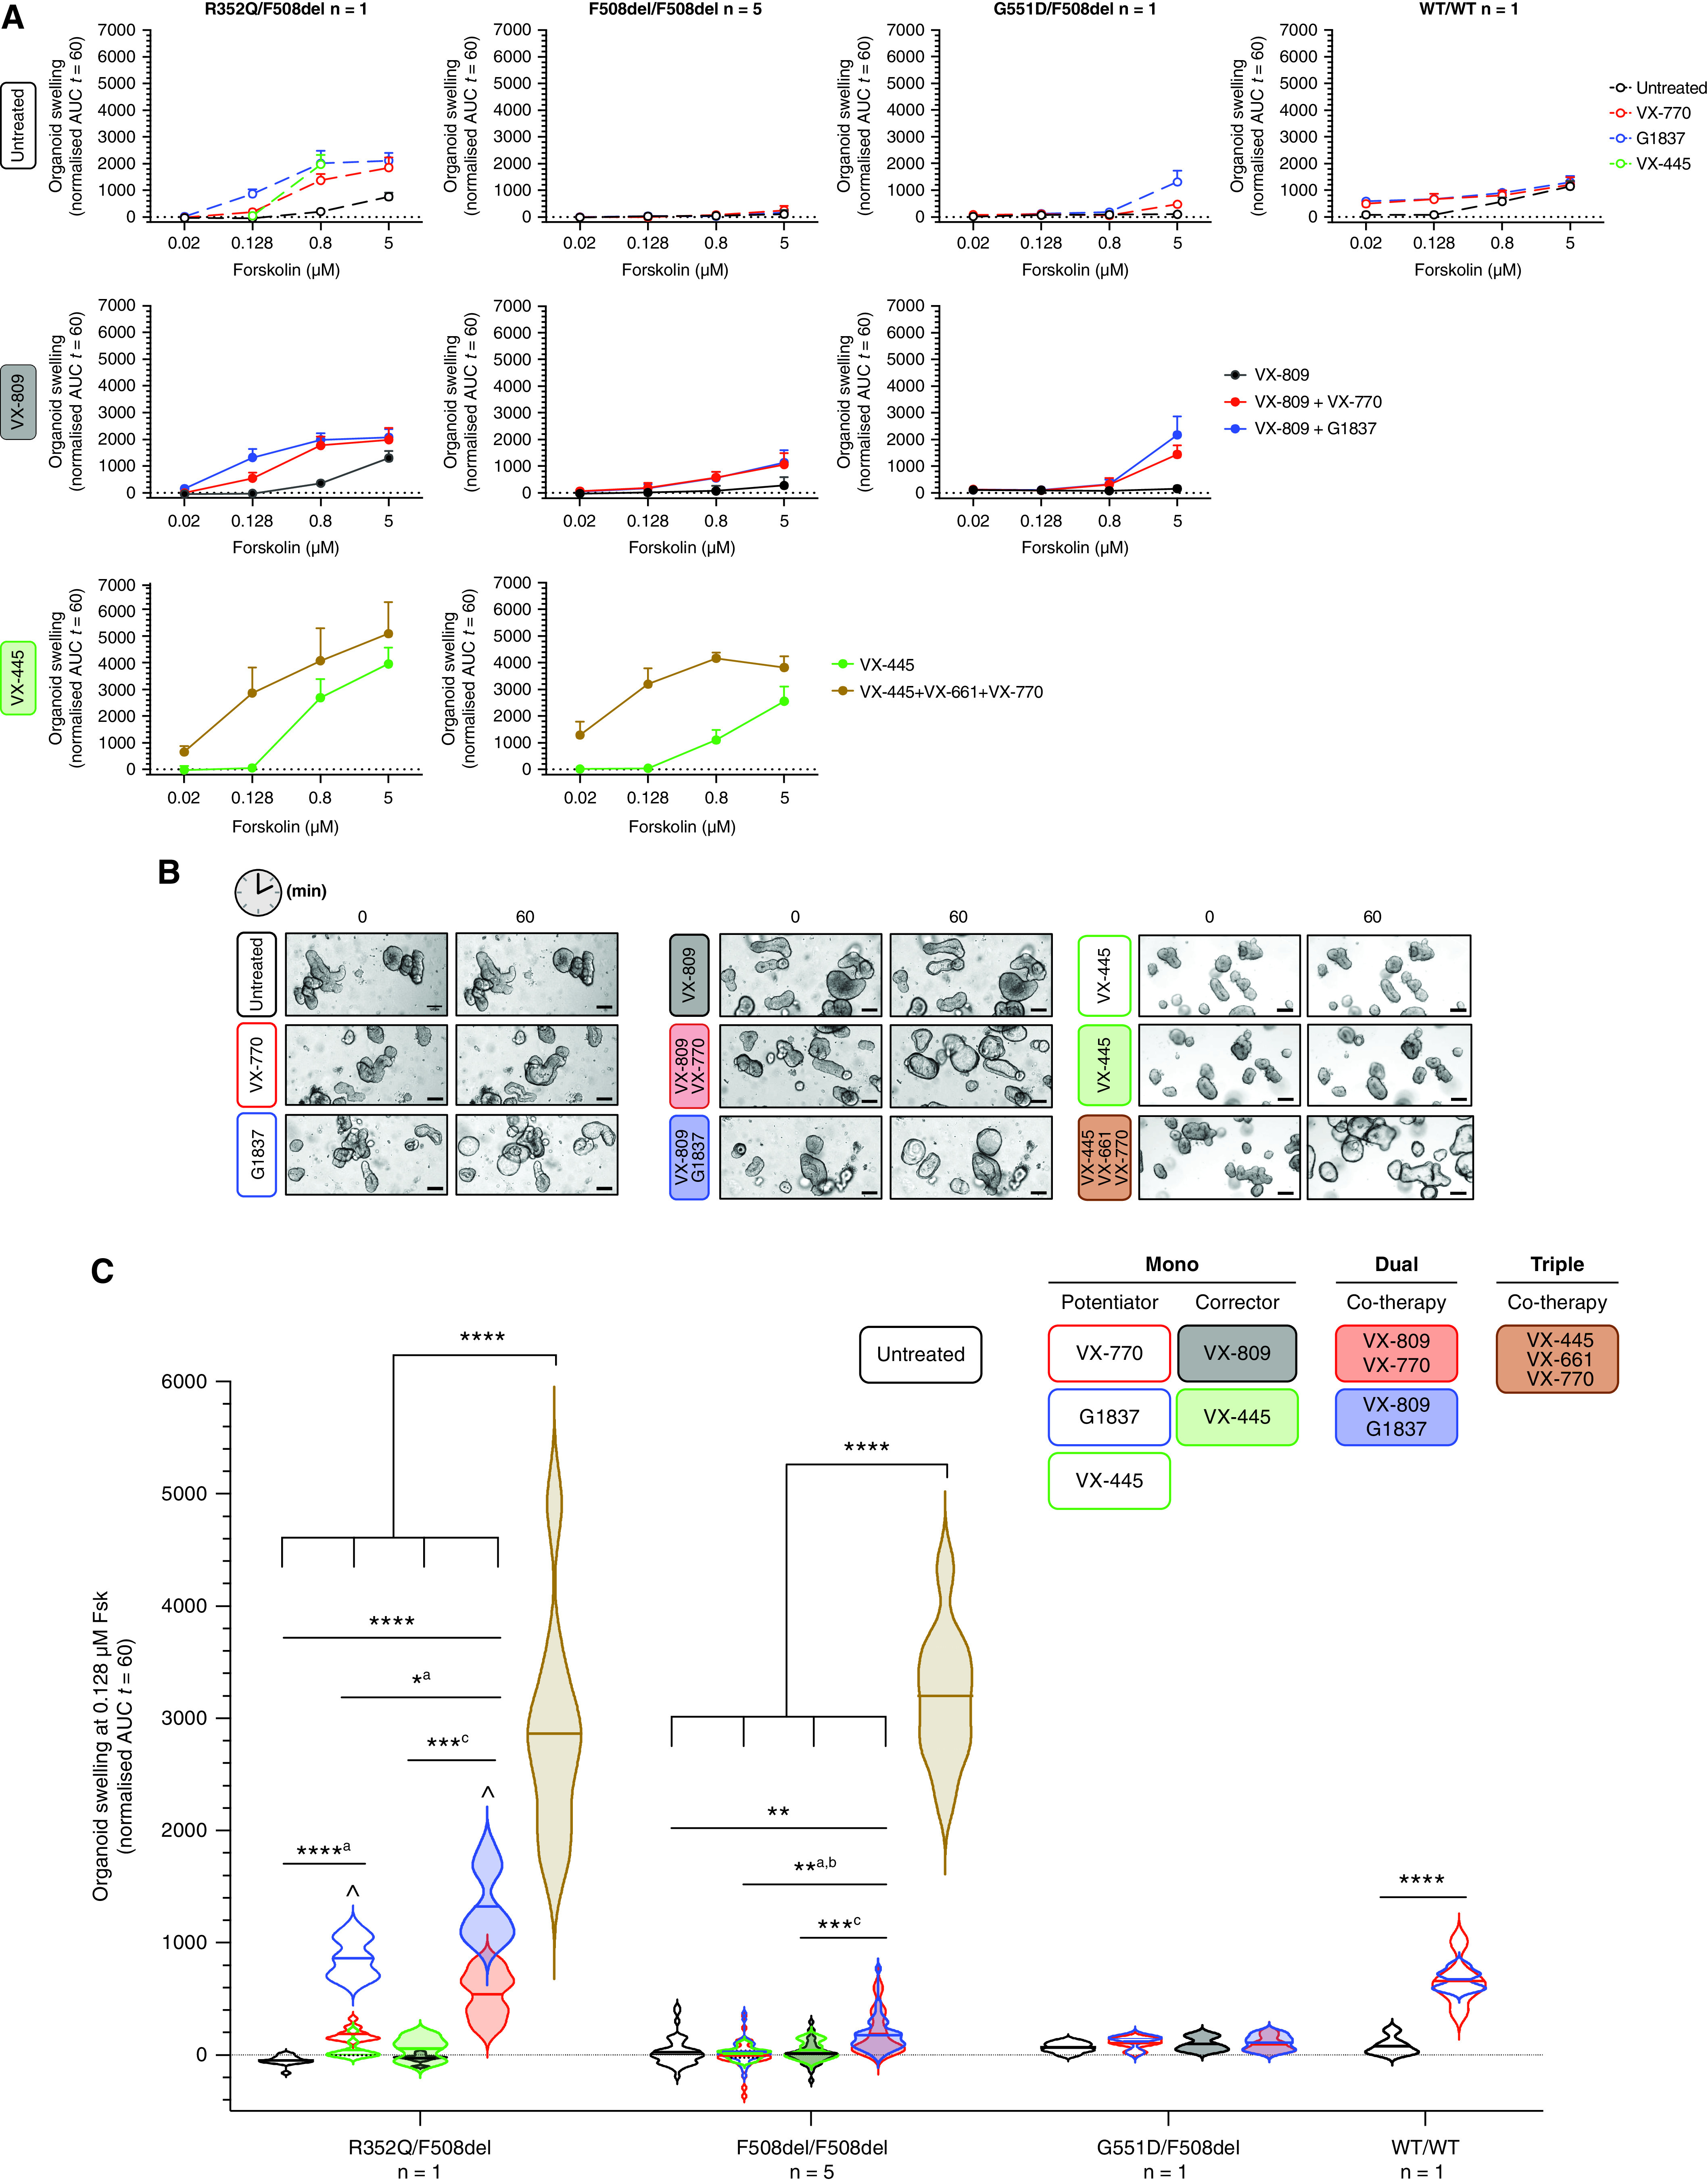
\includegraphics[width=0.80\textwidth]{figures/R352Q/figure_2.jpg}
	\label{R352_figure_1}
	\end{center}
	%\captionsetup{singlelinecheck = false, justification=raggedright}
	\begingroup
	\captionof{figure}[Functional response of R352Q-CFTR to CFTR modulators in intestinal organoids.] {\textbf{Functional response of R352Q-CFTR to CFTR modulators in intestinal organoids.}}{ Forskolin-induced swelling (FIS) assay in organoids (left to right) from one R352Q/F508del participant, five F508del/F508del participants, and one G551D/F508del participant with CF and one WT-CFTR control participant. Organoids were incubated overnight with 0.03\% DMSO (vehicle) or 3 $\mu$M VX-809 or 3 $\mu$M VX-445 or 3 $\mu$M VX-445 + 18 $\mu$M VX-661. After 24 hours, a range of Fsk concentrations from 0.02 to 5 $\mu$M were acutely added, either alone or in combination with 3 $\mu$M VX-770 (red) or 3 $\mu$M G1837 (blue) or 3 $\mu$M VX-445 (green). (A) Values plotted are the mean ± SD of the area under the curve (AUC). (B) Representative brightfield images of R352Q/F508del organoids at baseline (t = 0) and after 1 hour of stimulation (t = 60) at 0.128 $\mu$M Fsk. Scale bars, 100 $\mu$m. (C) Violin plots of FIS response (AUC at 0.128 $\mu$M Fsk) of organoids from participants with CF and WT-CFTR control participants, expressed as the absolute AUC calculated from the time periods t = 0 (baseline) to t = 60. Data are represented as violin plots to show the distribution of data. n, number of participants. One-way ANOVA was used to determine statistically significant differences. *P < 0.05, **P $<$ 0.01, ***P $<$ 0.001, and ****P $<$ 0.0001. aP for G1837 only, bP for VX-770 only, cP for VX-809 only, and \^P for G1837 versus VX-770 or VX-445. Where VX-770, G1837, and VX-445 (overlapping violin plots) achieved statistical significance, the least significant P value is shown.}
	\endgroup
%\end{figure*}

FIS of intestinal organoids at 0.128 $\mu$M Fsk has been demonstrated to correlate strongly with clinical modulator responses and therefore is used to assess CFTR modulator response in vitro \cite{dekkers2016}. At this Fsk concentration, organoids—independent of CFTR genotype—did not demonstrate FIS greater than AUC of 67.1 (Figures 2B and 2C, Table E3, Figure E2). In F508del/F508del organoids, treatment with either VX-770 or G1837 did not induce any swelling, suggesting no improvement in CFTR activity with potentiator therapy. G551D/F508del organoids showed a modest 1.5-fold increase in FIS after treatment with either potentiator, increasing AUC by 38.9 (VX-770) and 54.2 (G1837) above baseline (Figure 2C, Table E3). In WT/WT organoids, potentiation with both VX-770 and G1837 led to a significant (P $<$ 0.001) increase in FIS, increasing AUC by 580.6 and 594.2 above baseline, respectively (Figure 2C). In R352Q/F508del organoids, potentiation with either VX-770 or G1837 led to a significant increase in FIS, increasing AUC by 234.6 and 910.6 above baseline, respectively (Figures 2B and 2C). G1837 was significantly (P $<$ 0.0001) more effective in increasing FIS when compared with VX-770 in R352Q/F508del organoids, but not in organoids with the other CFTR genotypes, wherein the efficacy of the potentiators did not significantly differ from each other (Figure 2C, Table E3). Consistent with previous studies showing that VX-445 potentiates CFTR activity but is less potent than VX-770 (7–9), acute treatment of VX-445 modestly increased FIS in R352Q/F508del organoids by an AUC of 90.6 above baseline, lower than the AUC of 234.6 above baseline observed with VX-770 treatment (Figures 2B and 2C). As expected, acute treatment of VX-445 did not induce swelling in F508del/F508del organoids. These data indicate that R352Q has residual CFTR function and is responsive to VX-770 and G1837.

We next determined the effect of VX-809 monotherapy and cotherapy in R352Q/F508del organoids. In reference F508del/F508del and G551D/F508del organoids, VX-809 monotherapy at 0.128 $\mu$M Fsk concentration did not yield a significant change in FIS, with a net increase in AUC $\leq$ 30.4 above baseline (Figure 2C, Table E3, Figure E2). In F508del/F508del organoids, VX-809 cotherapy with either VX-770 or G1837 caused a significant (P $<$ 0.01) increase in FIS compared with potentiator monotherapy, with a net increase in AUC of 189.3 and 145.6, respectively (Figure 2C, Table E3). In contrast, no additional increase in FIS was observed in G551D/F508del organoids after cotherapy with VX-809 and either potentiator (Figure 2C). Similar to the reference F508del/F508del organoids, no change in FIS was observed in the R352Q/F508del organoids at 0.128 $\mu$M Fsk with VX-809 monotherapy. The net increase in AUC was 17.7 above baseline (Figures 2B and 2C, Table E3). VX-809 cotherapy in R352Q/F508del organoids followed the same trend as the F508del/F508del organoids but with a larger magnitude of response. VX-809 cotherapy with VX-770 or G1837 increased FIS beyond each respective monotherapy by 355.2 and 459.7 (Figures 2B and 2C).

The effect of VX-445 monotherapy as a corrector and VX-445+VX-661+VX-770 (Trikafta) triple combination therapy were tested in R352Q/F508del and F508del/F508del organoids. Similar to VX-809 monotherapy, VX-445 monotherapy at 0.128 $\mu$M Fsk induced minimal FIS in R352Q/F508del and F508del/F508del organoids, increasing AUC by 101.3 and 15.2 above baseline, respectively (Figures 2A–2C). In contrast, triple combination therapy VX-445+VX-661+VX-770 significantly induced FIS in R352Q/F508del and F508del/F508del organoids, increasing AUC by 2,913 and 3,173 above baseline, respectively. Because VX-445+VX-661+VX-770 primarily targets F508del folding and processing defects, the lower magnitude of CFTR correction in R352Q/F508del organoids than in F508del/F508del organoids supports our hypothesis that R352Q is unlikely to have folding and processing defects and that the functional correction observed is likely attributed to the F508del mutation.

\subsection{Correlation of CFTR Modulator Response in hNECs with Participant-matched Intestinal Organoid Swelling Assay Outcomes}

We compared the CFTR modulator response as determined by ion transport in hNECs and FIS in intestinal organoids. To determine the amount of modulator-stimulated restoration above the baseline CFTR activity, we subtracted the $\Delta$Isc/AUC values with Fsk alone from those with Fsk plus modulators. A linear positive correlation was observed (r = 0.75; P $<$ 0.0001) (Figure 3A). Participant-to-participant variability was evident (Figure 3B, Figure E3). Among the modulators, an inverse correlation was observed in response to VX-809 monotherapy between the two cell models (r = −0.74) (Figure 3C). Although VX-809 monotherapy significantly increased baseline currents in hNECs, no increase in FIS was detected in the matched organoids (Figure E3). When comparing CFTRinh-172–inhibited currents in hNECs against FIS in intestinal organoids, a similar trend of linear correlation was observed (r = −0.52; P $<$ 0.01) (Figures 3A–3C).

\subsection{Maturation of R352Q-CFTR in Nasal Epithelial Cells and Intestinal Organoids}

We next compared CFTR maturation in R352Q/F508del hNECs and intestinal organoids, with and without VX-809 treatment, to understand the distinct response of the two cell models to VX-809 monotherapy (Figure 3D). Robust expression of mature, complex-glycosylated CFTR at ~160 kD (band C) was detected in both untreated and VX-809–treated hNECs and intestinal organoids. Immature, core-glycosylated CFTR at ~130 kD (band B) was not present. This validates our functional data by showing the presence of mature CFTR channels on the cell surface in R352Q/F508del hNECs and intestinal organoids, which can therefore elicit residual CFTR function and also respond to potentiator (acts on protein at the cell surface). Mature CFTR in intestinal organoids migrated slightly farther (lower molecular weight) than the hNECs, likely because of different processes of CFTR glycosylation in different tissues, which has been reported previously \cite{vanbarneveld2010}. Treatment with VX-809 did not further increase the levels of mature CFTR relative to the untreated control in both hNECs (densitometry/×104 of 2.2 vs. 2.0) and intestinal organoids (densitometry/×104 of 2.9 vs. 3.1). This is consistent with the nonsignificant or lack of functional rescue with VX-809 monotherapy in R352Q/F508del hNECs and intestinal organoids, respectively. It is noted that the intestinal organoids expressed a higher abundance of mature CFTR protein relative to the hNECs (~1.5 times), consistent with known CFTR enrichment in the human gallbladder, intestine, and pancreas \cite{human_protein_atlas_2021, uhlen2015}.

\subsection{Molecular Dynamics Simulations and Free Energy Calculations Reveal the Dysfunction of the R352Q Mutant}


We next characterized the structural defect of R352Q-CFTR with molecular dynamics (MD) simulations, using an extended model of the phosphorylated, ATP-bound human CFTR \cite{wong2022}. In line with the previously proposed role for R352 in forming a salt bridge \cite{cui2008}, it was observed that mutation of the positively charged arginine (R) to neutral glutamine (Q) disrupted the R352-D993 salt bridge in the midsection of the CFTR channel pore (Figure 4A, Figure E4). This salt bridge is a key structural element in CFTR, and its disruption has been shown to impact conductance and gating \cite{cui2008}. However, there was no discernible disruption to the R352Q-CFTR channel pore architecture, because the root mean squared deviations of membrane-spanning helices of the R352Q-CFTR were as stable as the WT in microsecond-long MD simulations (Figure 4B). This suggests that the R352Q-CFTR open conformation can remain stable on the submicrosecond time scale necessary for chloride conduction \cite{sorum2015}. If gating was impacted by the R352Q mutation, longer simulations might be able to decipher any disrupted pore architecture.

Because the R352 residue lines the CFTR channel pore, the R352Q mutation can be expected to affect the conduction of chloride ions \cite{zhang2018}. This was assessed by determining the path of chloride conduction through the channel and comparing the occupancy of residues along the conduction pathway in WT-CFTR and R352Q-CFTR (Figures 4C and 4D, Video E2). In the WT system, a chloride ion spontaneously enters the pore intracellular gate \cite{linsdell2018} and diffuses toward K190 and K370 (site I) (Figure 4C). It remains in this site for ~10 nanoseconds and then spontaneously moves up to the vicinity of R352 and R303 (site II). R248, which is positioned between sites I and II, coordinates the chloride ion movement between these sites. The chloride ion then moves to the vicinity of R134 and K95 (site III), which coordinate chloride diffusion into the outermost section of CFTR. Chloride conduction through the CFTR channel pore does not follow a straight path from pore entry to site III but rather follows a longer, indirect route. This is in contrast to the straight path that ions follow through voltage-gated potassium and sodium channels, which have tight pores that run perpendicular to the membrane \cite{flood2019}.

In R352Q-CFTR, chloride ions can enter the channel pore but not as readily as in the WT system. They also generally do not progress as far into the pore as for WT-CFTR. Although multiple chloride ions occupied the WT-CFTR channel pore concurrently, only one chloride ion at a time was observed in the R352Q-CFTR channel pore. The highest occupancy in R352Q-CFTR was found for K1041. The chloride ions that enter the WT-CFTR channel pore stayed mainly in sites I and II, with occupancies of these two sites drastically reduced in R352Q-CFTR compared with WT-CFTR. This reduction in occupancy observed in R352Q-CFTR is due to neutralization of the positively charged R352 side chain, which reduces the affinity of chloride ions to site II. Site III was inadequately sampled to draw conclusions (Figure 4D). Intriguingly, some chloride ions appeared to penetrate site III in both WT- and R352Q-CFTR, which could explain the mild conductance defect observed for R352Q. In addition, in simulations of WT-CFTR, it was observed that D993 alternated contact between R303 and R352 (Figures E4A and E4B). However, in R352Q-CFTR, D993 forms a more stable salt bridge with R303 (Figure E4C), which curtails its ability to coordinate a chloride ion.

The impact of the lower occupancy of sites I and II on chloride conductance was quantified further by comparing the respective free energy profiles obtained from umbrella sampling MD simulations (Figure 4E). To generate the initial path for the umbrella sampling simulations, one chloride ion was constrained at site I and then steered via site II toward R134 in site III, using a moving restraint. The free energy profile calculations followed the protocol described in the Supplemental Materials and Methods of the data supplement. In WT-CFTR, calculation of the free energy profile yielded an energy trough of −4 kcal/mol at site II relative to site I (Figure 4E). This indicates that chloride ions will be attracted to this site. In contrast, in R352Q-CFTR, the free energy profile exhibited an energy barrier of +1 kcal/mol at site II, which will likely hinder chloride conduction. Therefore, in WT-CFTR, a chloride ion in site I will tend to move to site II, whereas such a motion will be suppressed in R352Q-CFTR, resulting in reduced chloride conductance.

\section{Discussion}
This study adds to previously published findings by other CF laboratories by validating the reproducibility of cell models created from participants with CF for assessment of CFTR activity via in vitro CFTR functional assays \cite{dekkers2016, ramalho2021}. To characterize the rare R352Q-CFTR mutation, we first created matched hNECs and intestinal organoids from participants with CFTR mutations that have known functional defects. These acted as references in the functional assays, and because these reference mutations are common to other published platforms \cite{dekkers2016, ramalho2021}, this facilitated comparison of data from our functional platform. Our reference hNECs and organoids both showed similar patterns of response to modulators when compared with previous studies, although the magnitude of response is lower \cite{dekkers2016, ramalho2021, pranke2017, pranke2019a}. Variabilities in the magnitude of CFTR response in cell models created from different laboratories are evident (Figure E5). This could be attributed to several reasons. First, CFTR functional response to modulators in patient cell models was shown to be significantly modified by minor alterations to the culture media \cite{gentzsch2017, saint-criq2020}. Patient-to-patient variability in CFTR response may also explain this observation \cite{pranke2017, matthes2018, brewington2018}, which could be further skewed if a relatively small number of participants are studied. The variabilities in data between laboratories highlight the necessity to create reference cell models at every test center for comparison and characterization of rare CFTR genotypes.

To date, R352Q-CFTR functional characterization has been performed only in heterologous expression Chinese hamster ovary, Fischer rat thyroid and CFBE41o− cells \cite{guinamard1999, vangoor2014,veit2020 }. These studies demonstrate varying levels of baseline activity ranging from 3\% to 20\% of WT-CFTR. However, in vivo CFTR function measured using nasal potential difference has shown that an individual with the R352Q/G1244E-CFTR genotype had CFTR activity just below that of WT individuals \cite{pranke2017}. The G1244E mutation is a CFTR gating mutation with severe defect \cite{cftr2}, suggesting that R352Q confers high levels of CFTR activity. To better characterize the R352Q mutation, we assessed CFTR function in hNECs and organoids derived from a R352Q/F508del-CFTR participant. Of the 100 individuals bearing the R352Q mutation in the CFTR2 database, 99 are heterozygous with F508del or another CFTR mutation genotype \cite{cftr2}. Therefore, our study participant is an appropriate representative of the R352Q-CFTR population.

The CFTR activity of a mutation is commonly expressed as a percentage of WT-CFTR activity to measure the severity of defect and responsiveness to modulator \cite{pranke2017,vangoor2014}. However, we noted limitation in its use because WT-CFTR activity is somewhat underestimated in hNECs, resulting in overestimation of mutant CFTR activity. Baseline CFTR activity in R352Q/F508del hNECs was 70\% of WT-CFTR activity. This was potentiated to well above WT-CFTR activity by VX-770 and G1837. Underestimation of the WT-CFTR activity was also shown by Pranke and colleagues \cite{pranke2017}, who showed that VX-770-potentiated CFTR current for R352Q/G1244E hNECs was \~160\% of the WT-CFTR activity \cite{pranke2017}. In our study, we found that the WT hNECs had significantly higher resting Isc than the CF hNECs (WT, 27.5 $\pm$ 1.5 $\mu$A/cm$^2$ vs. CF, 1.1 $\pm$ 0.7 $\mu$A/cm$^2$; P $<$ 0.0001; data not shown), suggesting that there was endogenous CFTR activity at resting state even without the presence of Fsk. This may have limited further chloride transport when the cells were stimulated with Fsk, underestimating the WT-CFTR activity. The presence of endogenous CFTR activity is also evident in WT intestinal organoids, which were reported to have preswollen morphology at resting state in the absence of Fsk \cite{dekkers2016}. Notably, a recent study reported that patient-derived cell models are effective tools to identify modulator-responsive patients but may not accurately predict the magnitude of clinical benefit \cite{kerem2021}. It is likely that although the percentage of WT-CFTR activity is useful as a guide of reference for CFTR functional rescue, in vitro and in vivo CFTR function do not correlate in a linear fashion.

Nonetheless, the high baseline Isc (14.8 $\mu$A/cm$^2$) and FIS (AUC, 196.3) of R352Q indicates a discernible amount of functional CFTR is present at the cell surface. In support of this, VX-809 monotherapy did not further improve CFTR activity in either R352Q/F508del hNECs or organoids. This is consistent with findings that VX-809 treatment did not further improve VX-770–potentiated CFTR activity in R352Q/G1244E hNECs \cite{pranke2017}. Western blot analysis in Fischer rat thyroid and CF bronchial epithelial cells showed that 80–98\% of R352Q-CFTR is present as mature CFTR localized to the cell surface, with little evidence of a processing or turnover defect \cite{vangoor2014, veit2020}. For this reason, because the mechanism of action of VX-809 is correction of a folding defect in CFTR that disrupts its trafficking to the cell surface, it is expected to have little, if any, restorative effect on R352Q-CFTR \cite{vangoor2011}. Our functional data confirm previous reports that the R352Q mutation is unlikely to cause folding defects and suggests that patients with R352Q-CFTR are unlikely to benefit from corrector modulator monotherapy.

Single-channel and whole-cell patch-clamp studies have demonstrated that the positively charged arginine (R352) creates an electropositive potential that promotes anion movement through the channel pore \cite{guinamard1999}. In addition, R352 forms a salt bridge with the negatively charged D993 residue (TM9), and this interaction is critical to keep the CFTR channel pore in a stable open-pore state \cite{cui2013a}. Our MD simulations performed on the extended structure of human CFTR (Protein Data Bank accession no. 6MSM) also showed that R352Q disrupts the R352-D993 salt bridge in the channel pore; however, the gross architecture of the channel pore was unchanged. We showed that the R352 residue is not essential for chloride ion entry into the channel pore but is necessary to maintain chloride ion occupancy at a binding site within the channel pore conductance pathway (site II) for normal chloride ion conductivity. This is consistent with previous studies demonstrating that R352Q caused frequent transitioning of the channel pore to subconductance states (\~40–70\%) and occasional full conductance channel pore opening \cite{zhang2017, cui2008}, causing a mild conductance defect. In the same studies, no apparent reduction in channel pore open probability (Po) was deduced or reported from the single-channel patch-clamp recordings, suggesting a gating defect was unlikely. This is consistent with our MD simulations that predicted the R352Q open conformer can remain stable during chloride ion conduction.

The exact mechanism of action of CFTR potentiators VX-770 and G1837 is not fully understood. There is evidence that VX-770 rescues gating defects by enhancing Po and stabilizing the open-pore conformation \cite{jih2017}. VX-770 was initially approved for CFTR gating defects \cite{fda_kalydeco_approval}. In some countries, approval has since been extended to conductance defects, based at least in part on in vitro functional assays \cite{vangoor2014, fda_kalydeco_2_years_or_older}. In principle, potentiators can enhance CFTR activity by increasing the opening time of channels (Po) and/or increasing channel conductance. It is plausible that the significant responsiveness of R352Q/F508del to potentiators was due to an increase in channel pore opening time. This extra time compensates for the energy barrier created by the R352Q mutation, which hinders chloride ion conduction.

Because CF is a multiorgan disease \cite{ratjen2015}. Overall, our data indicated a positive correlation between CFTR functional response to modulators in matched hNECs and organoids across all CFTR mutations assayed. This is consistent with recent findings in several other rare CFTR mutations, such as G85E, P205S, and D614G \cite{silva2021}. In our study, among all modulators, VX-809 monotherapy was the only therapy to result in a negative correlation in response between the two cell models in all participants. The hNECs of all participants were responsive to VX-809 monotherapy but not their intestinal organoids. We propose two mechanisms that could result in this discrepancy. First, the VX-809 incubation time of 24 hours in organoids is shorter than the 48 hours in hNECs. This could impact the number of F508del-CFTR that are successfully trafficked from the endoplasmic reticulum to the cell surface because this correction is a time-dependent process \cite{jurkuvenaite2010}. In addition to having a trafficking and gating defect, F508del-CFTR is less stable at the cell surface \cite{gentzsch2004}. Therefore, the shorter VX-809 incubation period in organoids may negatively impact CFTR stabilization at the cell surface.

Another mechanism could be the different concentration of Fsk used between the two assays. Both the Isc and FIS assays use Fsk to stimulate protein kinase A–dependent CFTR activation \cite{dekkers2013, gentzsch2017}. Protein kinase A increases channel Po in a dose-dependent manner \cite{cui2019}. FIS at 0.128 $\mu$M Fsk correlates best with in vivo lung function (percent predicted FEV1) and allows characterization of responses in organoids without reaching ceiling threshold (saturation) in high residual function CFTR mutations \cite{dekkers2016}. In contrast, 10 $\mu$M Fsk has been the default concentration for Isc measurements since early reports of this technique \cite{blouquit2002, smith1993}. However, it has recently been shown that 3 $\mu$M Fsk is sufficient to saturate the CFTR response in hNECs \cite{avramescu2017}. The high concentrations of Fsk in the Isc assay are likely to function like a potentiator, extending CFTR channel opening time \cite{cui2019}. This might explain the significant response to VX-809 monotherapy we observed in hNECs but not in matching organoids that were treated with a nearly 100-fold lower concentration of Fsk (0.128 $\mu$M).
Strengths and Limitations

A strength of our study is the cross-validation of modulator response in matched hNECs and intestinal organoid cultures derived from the same participants. This minimizes the possibility of cell culture–dependent bias. We could not correlate in vitro CFTR response to participant in vivo clinical response, because individuals under 12 years of age with an R352Q-CFTR mutation in Australia do not currently have access to CFTR modulator therapy.

MD simulation studies are emerging as a method to understand the molecular mechanism by which rare mutations cause the CFTR protein to misfunction \cite{callebaut2017}. The combination approach of using in vitro experiments and MD simulations to characterize the R352Q-CFTR mutation paves a feasible and reliable pathway to personalized therapies for participants with rare CFTR mutations (Figure 5). In our simulations, we demonstrated that alterations to the free energy profile in the channel pore introduced as a result of the R352Q mutation negatively impacted movement of the chloride ions to move past the midpoint of the CFTR channel pore (site II), diminishing the channel’s conductance. In vitro experiments complement these simulations by demonstrating that the unique defect introduced by a mutation can be rescued by CFTR modulators (61–63). In this study, we have demonstrated that the R352Q-CFTR defect is rescued by potentiators. Functional characterization of CFTR in both lung and intestinal models may improve the specificity and sensitivity of predicting modulator test results and aid in translating patient-derived cell models to become a mainstream companion diagnostic test for people with CF.
